\documentclass{beamer}
\definecolor{cadmiumgreen}{rgb}{0.0, 0.42, 0.24}
\usepackage[utf8]{inputenc}
\usetheme{Madrid}
\usecolortheme{rose}
\definecolor{coolblack}{rgb}{0.0, 0.18, 0.39}
\definecolor{UBCblue}{rgb}{0.0, 0.18, 0.39} % UBC Blue (primary)
\definecolor{UBCgrey}{rgb}{0.3686, 0.5255, 0.6235} % UBC Grey (secondary)
\setbeamercolor{palette primary}{bg=UBCblue,fg=white}
\setbeamercolor{palette secondary}{bg=UBCblue,fg=white}
\setbeamercolor{palette tertiary}{bg=UBCblue,fg=white}
\setbeamercolor{palette quaternary}{bg=UBCblue,fg=white}
\setbeamercolor{structure}{fg=UBCblue} % itemize, enumerate, etc
\setbeamercolor{section in toc}{fg=UBCblue} 
\setbeamertemplate{headline}{}
\setbeamertemplate{itemize items}[circle]
\setbeamertemplate{enumerate items}[default]
%\setbeamertemplate{footline}[frame number]
\setbeamertemplate{frametitle}[default][center]
\usefonttheme{serif}
% Packages
\usepackage[T1]{fontenc}
\usepackage{graphicx}
\usepackage{caption}
\usepackage{amsmath}
\usepackage{amsfonts}
\usepackage{amssymb}
\usepackage[main=english]{babel}
\usepackage{cite}
\usepackage{bookmark}
\usepackage{hyperref}
\usepackage{tikz}
\setbeamertemplate{navigation symbols}{}
\setbeamertemplate{bibliography item}{\insertbiblabel}



\title[TDAQ \& VST]{Collaboration Meeting: TDAQ Update}
\vspace{-3mm}
\author[Sara Gamba]{Sara Gamba (Unipi)\\ \\Pavel Murat (FNAL)}
\institute[Unipi]{\centering
\includegraphics[height=1cm]{FNAL-Logo-NAL-Blue.png}\hspace{10mm}\includegraphics[height=1.6cm]{cherubino_pant541.eps}}
\date[03/18/2024]{March 18th 2024}

\titlegraphic{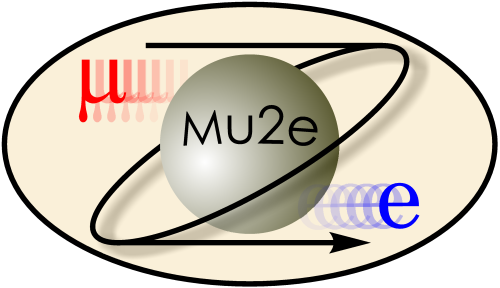
\includegraphics[height=1.6cm]{mu2e_logo_oval.png}\hspace{1.4cm}}
\begin{document}

\begin{frame}
\titlepage
\end{frame}
\begin{frame}{Working area}
    \begin{columns}
        \begin{column}{0.5\framewidth}
            \begin{figure}[H]
                \centering
                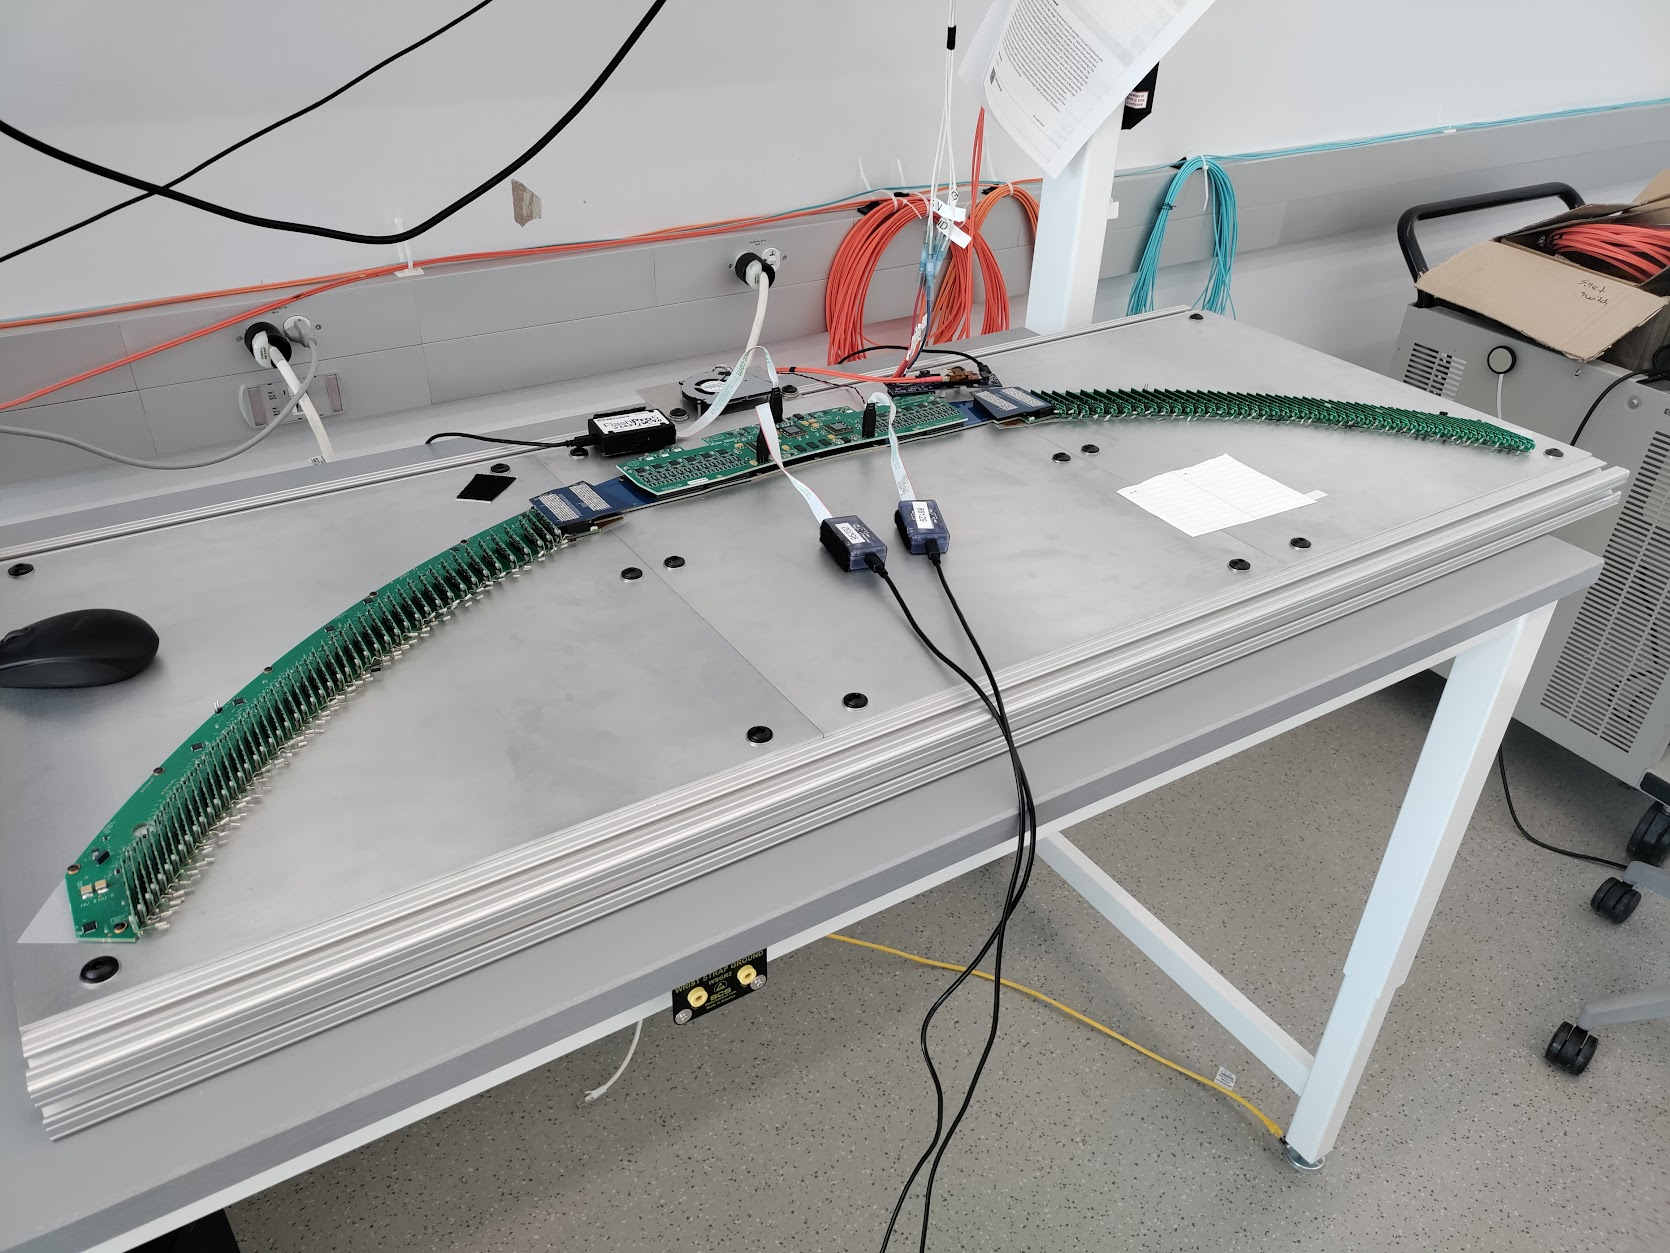
\includegraphics[width= \columnwidth]{IMG_20240219_090538.jpg}
                \label{fig:enter-label}
            \end{figure}
        \end{column}
        \begin{column}{0.5\framewidth}
            \begin{itemize}
                \item 3 test stands (IERC);
                \item A pulser implemented in the DRACs is sending pulses to the preamps (CAL side);
                \item The generator frequency is 50 kHz;
                \item Pulses are digitized at 40 MHz;
                \item Only 12 channels pulsed per RUN (one pulse every 8 channels);
                \item We are using 1 or 2 ROCs at the same time.

            \end{itemize}
        \end{column}
    \end{columns}
    \vspace{5mm}
    \textbf{Trying to understand failure modes and features of the boards}
\end{frame}

\begin{frame}{Waveforms}
    
\end{frame}
\end{document}
